\chapter{Background}
\label{chap:litreview}

This chapter summarizes linguistic and NLP literature in order to establish the role that interlinearization and morphological analysis has played in language documentation and description and how NLP work is related. The research explores ways to integrate machine learning, specifically for automating the three initial tasks of interlinearization (morpheme segmentation, morpheme glossing, and free translation) as well as inflectional paradigm induction. 

\section{Language Documentation and Description}
\label{sec:LDD}

The activities that constitute language documentation and language description fieldwork are not clearly distinguished. \citet{himmelmann_documentary_1998} defines language documentation as ``a comprehensive and representative sample of communicative events [that are] as natural as possible.” \citet{woodbury_defining_2003} defines it similarly as “comprehensive and transparent records supporting wide ranging scientific investigations of the language.” Language description can be defined as work that analyzes language documentation to create “systematic presentations of the phonology, morphology, syntax, and semantics of the language” \citep{bird_machine_2012}. The emphasis in linguistics on endangered languages over the past three decades has established modern field methods for recording and analyzing data \citep{bowern_linguistic_2008,czaykowska-higgins_research_2009,lupke_data_2010,vallejos_integrating_2014,rice_community-based_2017}. However, the specific activities that divide the two subfields are not rigid. Therefore, the currents work rarely distinguishes the two. Instead, it refers to the two together as “language documentation and description” or “documentary and descriptive linguistics”.

The workflow of language documentation and description activities is not standardized, although most projects seem to follow a similar sequence.  One common sequence of activities was described by \citet{bird_machine_2012}. A version is given below with numbers added which will be used in the following paragraphs to refer to each task (e.g. ``task 2a'' refers to the process of transcription). Bird and Chiang classify this workflow under language documentation, but each subsequent task progressively encompasses more description than documentation, excepting archiving, which comes strictly under language documentation but is logically the last step.

\begin{enumerate}
    \item Collect (audio/video recordings of) naturally occurring speech
    \item a) Transcribe and b) translate the recordings
    \item Perform basic morphosyntactic analysis of the transcription by segmenting the morphemes and creating morphological glosses and/or a lexicon
    \item Elicit morphological paradigms that will allow the study of specific phenomena and/or reveal underlying patterns
    \item Prepare a grammar of the language i.e. descriptive reports that outline how the language is structured
    \item Archive data in a long-term digital repository
\end{enumerate}

One primary output of this workflow is interlinear glossed texts (IGT), a distinctive data format in linguistics. 
%The process of creating IGT is interlinearization. 
Interlinearization takes center stage after recorded speech has been transcribed and moves the workflow beyond simple collection of data but still serves as a ``preprocessing step'' to \citep{moon_unsupervised_2009} language description (strictly defined). It comprises a number of annotation tasks that enrich the data with analytic information which can be added on lines under the original transcribed text. Several common lines of annotation are shown in Figure \ref{fig:IGTillus}. Interlinearizing more and more data uncovers the rarer and unique linguistic phenomena. To assist the identification and study of these phenomena other lines of annotation, such as lexical categories (POS tags), are added. The lines can be added in any order, but translations (task 2a) morpheme boundaries and morpheme glosses (task 3) are usually added first. As the workflow above indicates, descriptive annotation beyond these lines is beyond the priorities of language documentation (strictly defined). Therefore, in this work ``interlinearization'' usually denotes three annotation tasks: 1) identifying morpheme boundaries (\emph{morpheme segmentation}), 2) labeling each morpheme with its lexical meaning or morphosyntactic function (\emph{glossing}), and 3) providing \emph{free translations} of sentences in a language of wider communication.  

%The result is illustrated in example (\ref{ex:IGTex}) with a transliterated %Russian sentence.   

%\begin{singlespace}
%\pex<IGTex>   
%\label{ex:IGTex}
%\textbf{Text:} \hspace{14 mm} Vecherom \hspace{4.75 mm} ya \hspace{13 mm} pobejala \hspace{21 mm} v \hspace{2 %mm} magazin \\
%\textbf{Segmented:} \hspace{2 mm} vecher-om \hspace{4 mm} ya \hspace{13 mm} pobeja-la \hspace{20 mm} v \hspace{2 mm} magazin \\
%\textbf{Glossed:} \hspace{8.5 mm} evening-\textsc{ins} \hspace{1 mm} 1.\textsc{sg.nom} \hspace{1 mm} run-\textsc{pfv.pst.sg.fem} \hspace{1 mm} in \hspace{1 mm} store.\textsc{acc} \\
%\textbf{Translation:} \hspace{1 mm} `In the evening I ran to the store.' \\
%\xe
%\end{singlespace}

%This process makes documentation and description difficult to distinguish because it does not clearly fall under either subfield. 

\begin{figure}[!tb]
    \centering
    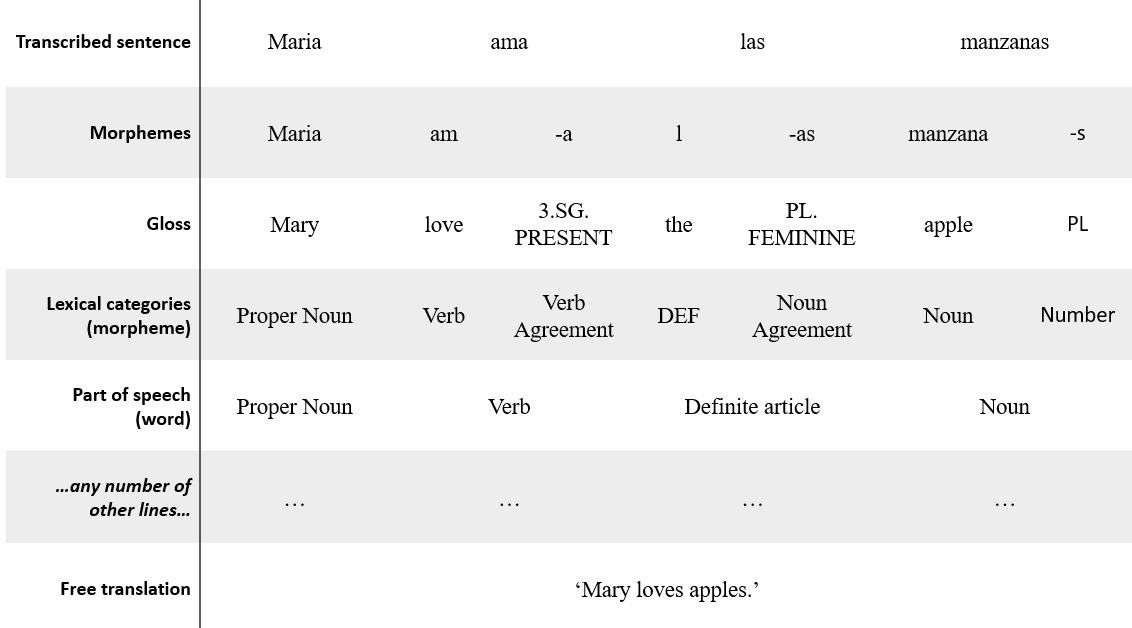
\includegraphics[width=15cm]{figs/IGT-illus.png}
    \caption[Interlinearization]{Interlinearization. Interlinear glossed texts add lines of annotation to the original text.}
    \label{fig:IGTillus}
\end{figure}

Interlinearization opens the door for deeper linguistic analysis and lays the foundation for reference grammars, dictionaries, and language learning materials, but interlinearizing naturally-occurring speech is not sufficient by itself to create complete grammars, dictionaries, etc. One additional descriptive task is often included during the fieldwork stage of the workflow: the collection of morphological inflection patterns, or paradigms, for several lemmata (task 4). Inflectional paradigms are elicited in documentary work because complete paradigms are rarely found in natural language. Complete lemma-specific paradigms are needed to infer general rules of inflection which are an important part of any systematic linguistic description.


\section{Natural Language Processing (NLP) for Low Resource Languages}

Though the line between language documentation and description may not be clear, one thing is clear: current methods do not scale up well. Documentary and descriptive projects often archive only partially accessible corpora, meaning that only a part of the corpus has any annotation beyond transcription. Without annotations such as translations, morpheme segmentation, and glossing, the documented and transcribed data is only understandable to someone who already speaks the language. If no speakers are left, the data is inaccessible, much like Egyptian hieroglyphics before the Rosetta Stone was discovered. Corpora are only partially annotated simply because funding and time are often not sufficient to complete interlinearization \citep{cox_taking_2019}. Current methods assume primarily manual work which is prone to human error and inconsistencies. Baldridge, Palmer, and others note that manual work is extremely inefficient and that the typical strategy of annotating texts from top to bottom is non-optimal for training a supervised machine learning model \citep{Baldridge06,baldridge_how_2009,palmer_semi-automated_2009}. Since naturally-occuring speech contains many repeated linguistic structures, manual annotation has been described as repetitive, monotonous, costly, and time-consuming \citep{duong_natural_2017,he_humanloop_2016}. For example, it can take anywhere from 20 to 100 hours to transcribe (task 2a) a single hour of speech \citep{seifart_language_2018}. It is reasonable to assume that interlinearization (tasks 2b and 3) and eliciting morphological paradigms (task 4) each require  significantly more time than transcription.  
%The problems with manual annotation is not limited to field linguistics; even a project for natural language processing required three years to annotate just one layer of the Penn Treebank \citep{taylor_penn_2003}. 
%accessible endangered and low-resource language data increases slowly and is plagued by quality issues. 

A few software tools specially designed for linguistic annotation do provide limited automated assistance for language documentation and description. The two most popular are ELAN \citep{auer_elan_2010} and FLEx \citep{rogers_review_2010}. Examples of their interlinearization interfaces are shown in Figures \ref{fig:FLEX} and \ref{fig:ELAN}. These tools perform automatic morpheme segmentation and glossing by implementing morphological parsers. The parsers require morphological rules that are created by hand. Such parsers do not generalize to new data. In addition to a parser, FLEx has a feature that copies morpheme boundaries and glosses onto new words, but only if the words are identical to words that were previously annotated by hand. Neither tool incorporates machine learning. 

\begin{figure}[!tb]
    \centering
    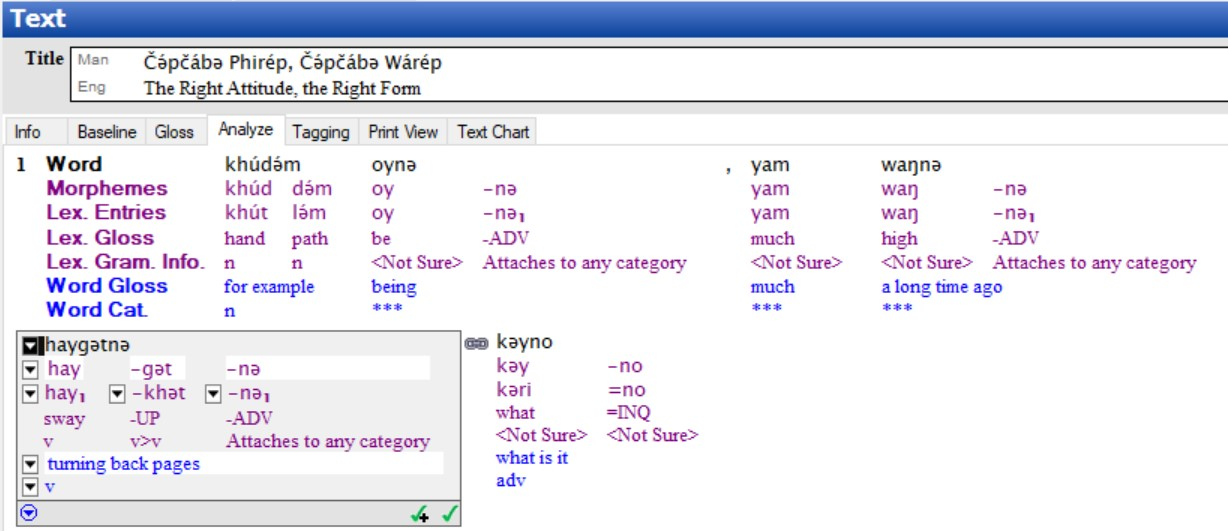
\includegraphics[width=15cm]{figs/ManipuriFLEx.jpg}
    \caption[FLEx]{User interface for interlinearization in Fieldworks Language Explorer (FLEx) displaying a Manipuri text in the corpus described in Chapter \ref{chap:datamodels}}
    \label{fig:FLEX}
\end{figure}

\begin{figure}[!tb]
    \centering
    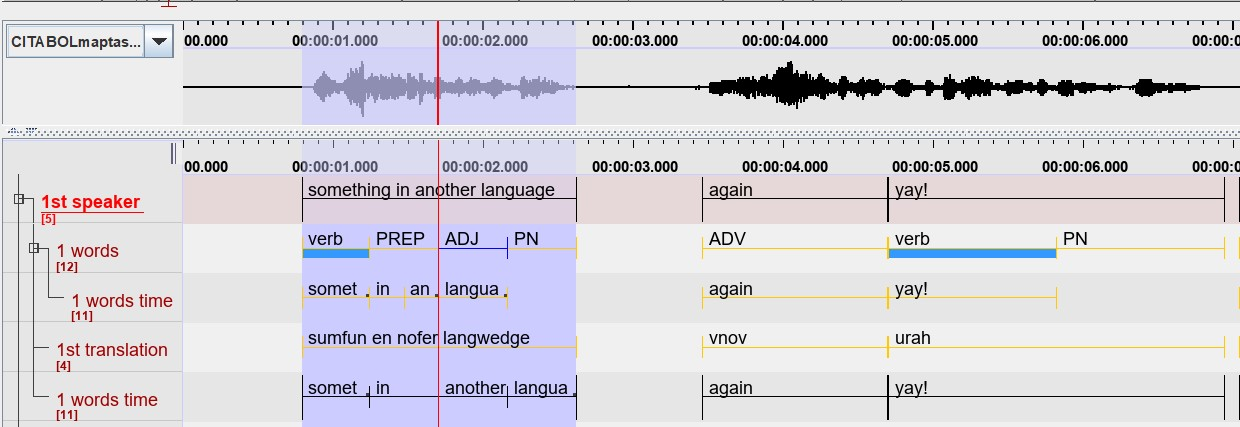
\includegraphics[width=12cm]{figs/ELANeng.jpg}
    \caption[ELAN]{User interface for interlinearization in ELAN showing a practice session in English.}
    \label{fig:ELAN}
\end{figure}

%The issues due to manual methods in language documentation and description could be avoided by integrating machine learning into the workflow. With the exception of audio/video recording, each task in Chiang and Bird’s workflow could be sped and improved with better automated assistance. Machine learning assistance could generate many more hours of transcribed speech in less time and many more lines of annotated text with fewer inconsistencies. Unfortunately, machine learning is not accessible to linguists without specialized training in NLP.

%Such annotated text supports deeper linguistic inquiry, the expansion of NLP, and the development of human language technology for low-resource languages.

%Since 2016 the CoNLL-SIGMORPHON shared tasks increased their list of languages from a couple dozen to over 100. This list is good benchmark of how much NLP interest in low-resource languages has grown recently. 

A recent growth of interest in low-resource languages\footnote{According to LORELEI (https://www.darpa.mil/program/low-resource-languages-for-emergent-incidents), ``low-resource'' refers to languages for which no automated human language technology exists. This is due to a lack of linguistic resources. \citet{szymanski_morphological_2012} estimates that 99\% of the world's languages are ``resource-poor''. In linguistics, it is more common to hear other terms. The current work uses the term ``under-described languages'' to refer to languages with minimal published linguistic resources; these have been called ``very scarce-resource language'' \citep{duong_natural_2017}. The term ``under-documented languages'' (Duong's ``extremely scarce-resource languages'') refer to languages that lack sufficient raw or annotated data to write a full reference grammar. The term ``endangered languages'' refers to languages that are predicted to have no native speakers within a generation or two. Most endangered languages are under-documented and/or under-described, as well as fitting the definition of low-resource languages. The distinctions between the terms are rarely crucial in the current work. In practice, these terms can be used almost interchangeably. } 
has developed models and methods that improve machine learning results with limited data. This includes machine translation \citep{abbott_towards_2018,gu_universal_2018,shearing_improving_2018,al_mumin_neural_2019,duh_benchmarking_2020}, computational morphology \citep{ruokolainen_supervised_2013,baumann_using_2014,micher_improving_2017,moeller_improving_2019}, syntactic parsing \citep{baldridge_learning_2013,duong-etal-2015-low,duong_natural_2017}, and automatic speech recognition \citep{adams_automatic_2017,anastasopoulos_computational_2019}. Several experiments have demonstrated that these models and methods are both practicable and beneficial for language documentation and description. Machine learning has already been leveraged to develop tools to automate transcription of documentary and descriptive audio recordings. A notable example is ELPIS \citep{foley_elpis_2018}, an online tool that includes a user interface accessible to those with no programming background. Machine translation (MT) has been applied to documentary data, using the output of an automatic speech recognition system as input to the MT system \citep{anastasopoulos_unsupervised_2016,duong_attentional_2016}. The potential for integrating machine learning into interlinearization has been clearly demonstrated \citep{baldridge_how_2009,palmer_semi-automated_2009,palmer_computational_2010,xia_enriching_2016}. For example, \citet{felt_improving_2012} found that automated ``pre-annotation'' improves human annotators' accuracy if the machine learning model achieves only 60\% accuracy and significantly speeds human annotation with an accuracy of 80\%. In the area of morphological paradigm induction, the annual SIGMORPHON and CoNLL-SIGMORPHON shared tasks \citep{cotterell_sigmorphon_2016,cotterell_conll-sigmorphon_2017,cotterell_conllsigmorphon_2018,mccarthy-etal-2019-sigmorphon} have developed many successful methods to improve learning of inflection with limited training data. 

Although NLP interest in low-resource languages has grown noticeably in the past few years, it is not a new area of research. Since the late 20\textsuperscript{th} century, NLP has taken several approaches to low-resource languages. These approaches can be classified as either rule-based (i.e. finite state transducers) \citep{cotterell_labeled_2015,forsberg_learning_2016,moeller_neural_2018,moeller_improving_2019} or machine learning that ``learn'' rules from data. Machine learning approaches to low-resource languages can be further divided into three types according to whether the training data was annotated completely (supervised) \citep{bergmanis_training_2017,sudhakar_experiments_2017,makarov_align_2017,liu_morphological_2018,makarov_uzh_2018}, partially (semi-supervised) \citep{ahlberg_semi-supervised_2014}, or not at all (unsupervised) \citep{moon_unsupervised_2009,palmer_computational_2010,kirschenbaum_unsupervised_2012,soricut_unsupervised_2015}. 

At first glance, unsupervised and semi-supervised learning seem most promising for language documentation and description because they do not require large amounts of manually annotated data as input. However, even though supervised learning requires annotation, it needs much less data than unsupervised learning and almost always yields better results \citep{ruokolainen_supervised_2013,cotterell_labeled_2015}. Additionally, without annotated labels, unsupervised learning can only really cluster data by the latent patterns in the data. Discovering latent patterns might be quite useful for linguists when first exploring the data; for example, frequent character patterns and substrings that a model discovers could provide an initial hypothesis to the linguist about the language's morphological structure. However, no matter how accurate an unsupervised model may be, it cannot substitute the valuable process of manually analyzing and discovering patterns in the data. Detailed analysis of new data is vital for linguists because through that process the linguist becomes familiar with the data and begins to absorb an intuitive knowledge of the language. Nevertheless, the latent patterns discovered by unsupervised models can have many uses such as being leveraged in a semi-supervised approach. Semi-supervised learning combines some supervised data with a larger set of unsupervised data   \citep{kohonen_semi-supervised_2010,poon_unsupervised_2009}. This approach may be more suitable than supervised learning if available annotated data is not adequate to effectively train a supervised model. 
Semi-supervised learning may be ideal for language documentation and description because having large amounts of unannotated data with a small amount of annotated data is a common situation, due to the annotation bottleneck. However, like unsupervised learning, semi-supervised learning requires some strong initial hypothesis about the data. These assumptions may hold true in pre-processed datasets but ``tend to be violated in real-world data'' \citep{druck_reducing_2007}. Unfortunately, real applications of semi-supervised learning, specifically for computational morphology, are relatively rare, particularly with neural networks. There are exceptions, such as \citet{ahlberg_semi-supervised_2014}, where semi-supervised learning was used to induce morphological paradigms in low-resource settings. 
%In addition, unannotated and annotated data cannot be simply combined together. Annotated data has to be weighted so that the larger, unannotated part does not overwhelm it. 

%\Mans{Also, unsupervised learning (with the possible exception of segmentation) is really all about clustering. What a language documentation project would do with that is unclear. I can imagine perhaps a morphological clustering of forms (hopefully under the same lemma) could be useful as a first step in trying to produce paradigms, but otherwise unsupervised learning is really limited in this context.}

%\Mans{Semi-supervised learning deserved a note. What if you could take a small number of annotated data and make clever use of the unannotated data to boost your accuracy? That could potentially be helpful. I haven't seen this done with neural models yet (although Ling \& I are working on it), but e.g. Ahlberg, Forsberg, Hulden (2014) is such an approach.}


%Supervised approaches developed later than unsupervised learning, due in part to computer memory limitations \citep{hammarstrom_unsupervised_2011}. Supervised neural networks, or deep learning, developed even later.

Supervised learning is trained on ``gold standard'' annotated data. It learns the patterns of the annotation labels. A successful model can label new data instances with high accuracy. The new data instance might be a morpheme segment, morpheme gloss, or translation of a word or phrase that was not present in the training data. 


%Having a gold standard makes supervised machine learning qualitatively different from unsupervised learning since unsupervised learning classifies data points into categories or classes.  

Until the 2010s, most machine learning models were feature-based with hand-designed features, illustrated in Figure \ref{fig:Features-ML}. 
%\mans{I think what you want to say is that until the 2010s the feature-based models all had hand-designed features.} 
A hand-designed feature function for a task such as morpheme segmentation might have 1) the whole word, 2) the position of the word in the sentence, 3) surrounding words or morphemes, 4) the POS tag of the previous morpheme/word. Features are assigned weights by the model during training in order to achieve optimal performance according to some objective function such as classification accuracy. These weights put the model's attention on the most helpful features for accurate performance. For example, in a morpheme segmentation task where one chosen feature is the previous word and the previous word is some form of the English ``to be'' verb, and the target word ends in ``ing'', then the model might give a high weight to the previous word so that the model pays attention to it when deciding how to segment a word ending in ``ing''. 
%If glossing is treated as a separated task, then the CRF might decide a word-final ``s'' marks a plurality---not 3rd person singular simple present tense---if during training it decided to give high weight to the POS tag. 

The performance of feature-based models, such as the CRF and SVM (see Chapter \ref{chap:datamodels}), relies heavily on the manual choice of features. This could be a drawback for under-described languages, because if little linguistic description is available, how does one know which features are optimal for that language? Fortunately, some feature-based models have been shown to perform reasonably well using language-independent features \citep{ruokolainen_comparative_2016,moeller_automatic_2018}.  

\begin{figure}[t]
\label{fig:Features-ML}
\begin{center}
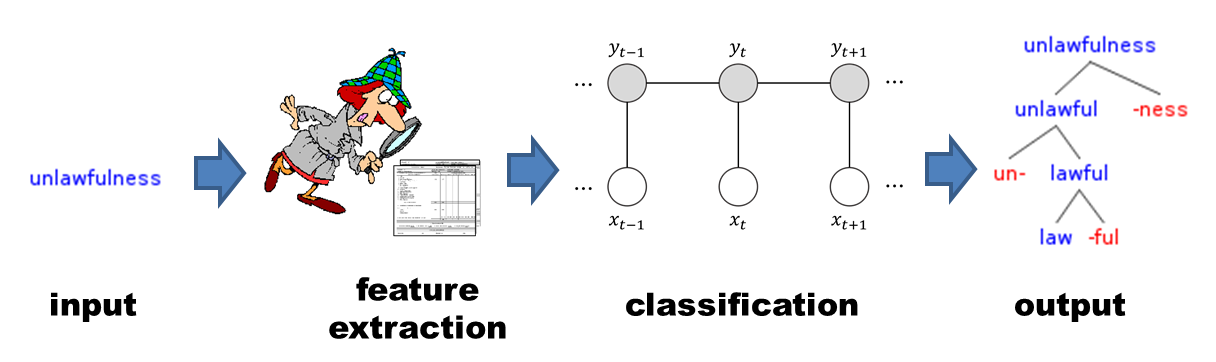
\includegraphics[width=0.95\columnwidth]{figs/Features-ML.PNG}
\caption[Feature-based machine learning]{Feature-based machine learning.}
\end{center}
\end{figure}

%\Mans{I think the below paragraph has the appropriate depth. However, maybe the crucial role of feature ``learning'' through having hidden layers gets lost in there somewhere. That is really the key part and why people say that NNs don't require manual feature design - you do require feature design (e.g. words), but they can be simpler and the NN can figure out a better representation for them because of the embedding layers. Could cite Bengio's language model paper from 2003 ``A Neural Probabilistic Language Model'' which contains the key insight ``learning a distributed representation for words which allows each training sentence to inform the model about an exponential number of semantically neighboring sentences''}

Currently, neural networks models, or deep learning models,
%that allow for end-to-end learning, but it's not really the same thing}
are dominating NLP \citep{goldberg_neural_2017}.
Even though they outperform older, feature-based models on almost all tasks, they did not become popular until the mid-2010s because they require greater computing power and, for some tasks, train more slowly \citep{cotterell_cross-lingual_2017}. Neural networks, illustrated in Figure \ref{fig:DL}, refers to a family of supervised machine learning models that are composed of layers of statistical units. The layers essentially substitute the feature engineering needed in non-neural machine learning. Multiple embedded layers allow the model to look at an exponential number of ``semantically'' neighboring instances of each training instance it encounters \citep{bengio_neural_2003}. The layers create intermediate representations of the data that allow the model to ``learn'' a distributed representation of elements within each instance (e.g. a distributed representation of words within a sentence). This ability of the model to learn requires no (or at most, very simple) manual feature design. Each unit in each layer is connected to each unit in the adjacent layers. Vector representations of the data are received by an input layer and transformed in ``hidden'' layers. The hidden layers feed into a final logistic function layer (i.e. softmax) that outputs a prediction of each possible class as a probability between 0 and 1. The connections between layers are represented by learnable weights; the higher the weight the more influence a unit has on the result. Since deep learning is supervised\footnote{Deep learning morphological segmentation has been performed on unsupervised texts with some success \citep{wang_morphological_2016}} the weights are adjusted with feedback from the gold standard. This is done via stochastic gradient descent or some similar optimization algorithm \citep{goldberg_neural_2017} with backpropagation that tells the model how to change the parameters which build the representation of each layer from the previous layer \citep{lecun_deep_2015}.

\begin{figure}[t]
\begin{center}
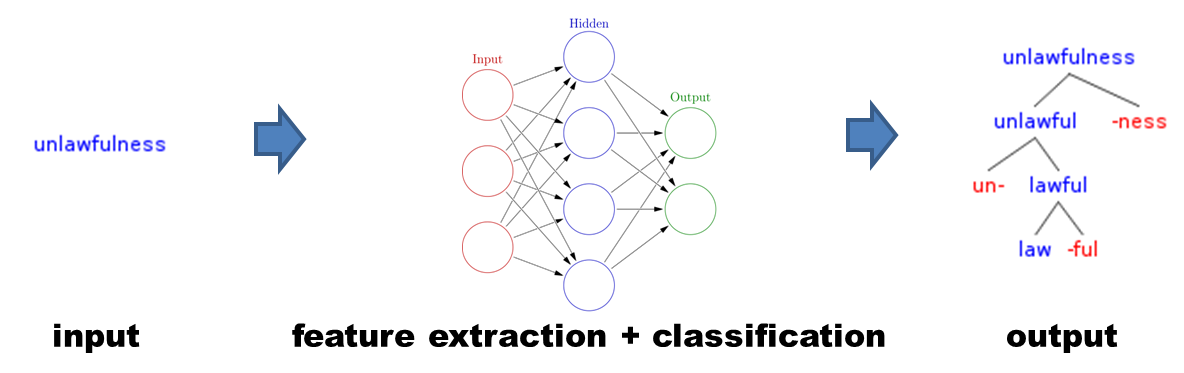
\includegraphics[width=0.95\columnwidth]{figs/DL.PNG}
\caption[Neural Networks
]{Neural Networks.}
\label{fig:DL}
\end{center}
\end{figure}

%Many flavors of neural machine learning exist and different models work best for different tasks. Encoder-decoders neural networks work well for mapping one sequence to another by encoding the input sequence of symbols (e.g. the letters of a word) and decoding it as another sequence of symbols (e.g. glosses). Encoder-decoders can be used for for morphological tagging \citep{heigold_extensive_2017}, segmentation (including low resource settings) \citep{kann_fortification_2018}, paradigm completion \citep{cotterell_conllsigmorphon_2018}, and translation. For example, morphological generation produces fully inflected forms from morphosyntactic or contextual information \citep{cotterell_conll-sigmorphon_2017} or completes morphological paradigms \citep{malouf_generating_2016}. 

Until recently, neural networks had the same great disadvantage for language documentation and description that unsupervised learning has. Good performance required a great deal of data. Until recently data from language documentation and description would have been considered inadequate to train neural networks \citep{duong_natural_2017}.
%Although neural models such as the Transformer generally outperform non-neural models, this does not necessarily hold true. 
Even now, a non-neural model can outperform any given neural model that is not tuned to low-resource settings, yet neural models can be difficult to optimize and tune for low resource settings \citep{popel_training_2018}.
Low-resource settings do not always respond to methods that are often effective for improving neural models. For example, fine-tuning hyperparameters or adding hidden layers may sometimes reduce accuracy with smaller amounts of data \citep{cotterell_conll-sigmorphon_2017,popel_training_2018}. 
%Pre-set or recommended hyper-parameters in NMT toolkits such as OpenNMT have been optimized for large datasets with millions of sentences and tend to hurt performance in low-resource settings. 

New methods are being developed that overcome neural models' dependence on large corpora. Methods include fine-tuning a model to the specific task and input data, training intermediate steps, or augmenting the training data.
%With such methods, neural models are beginning to outperform feature-based models even in low-resource settings.
\citet{van_biljon_optimal_2020} looked at fine-tuning a model for limited data and determined that shallow- or medium-depth size Transformer models, for example only 3 encoder and 3 decoder layers, give better results at tasks with limited training data. An example of an intermediate training step would be first training a segmentation model to produce surface morpheme breaks and the learn underlying forms of morphemes (e.g. ``impossible'' $\rightarrow$ ``in-possible'' $\rightarrow$ ``\textsc{neg}-possible'') \citep{liu_morphological_2018,moeller_improving_2019}. An similar strategy could be used in machine translation by first training the model to produce glosses and then ``translating'' the glosses into a more correct version of the target language (e.g. from Russian to English: Vecherom ya pobejala v magazin. $\rightarrow$ evening-\textsc{ins} \textsc{1.sg.nom} run-\textsc{pfv.pst.sg.fem} in store.\textsc{acc} $\rightarrow$ In the evening I ran to the store).

Another successful method is augmenting the training data. 
Data augmentation can be done with artificial word forms \citep{liu_morphological_2018} or with information extracted from other resources such as grammars and dictionaries. Leveraging multiple resources to train machine learning models is not impractical if language documentation and description projects have been undertaken in the language. Traditionally, documentary and descriptive projects produce some form of the Boasian triad, illustrated in Figure \ref{fig:Triad}. 

\begin{figure}[!tb]
\begin{center}
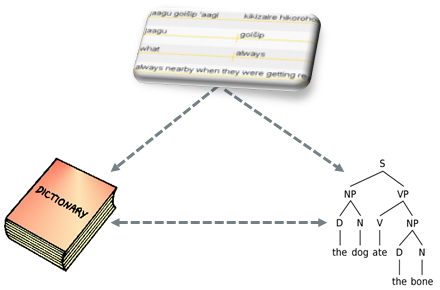
\includegraphics[width=8cm]{figs/Triad.PNG}
\caption[The Boasian Triad]{The Boasian Triad is a grammatical description, a bilingual lexicon, and a corpus of IGT.}
\label{fig:Triad}
\end{center}
\end{figure}


NLP research in low-resource languages has been growing quite a bit in the past 5-6 years, but most research has been applied to tasks relevant relevant to common NLP goals such as learning to predict unseen inflected forms, and very little has been applied to linguistic research such as discovering and describing the inflectional classes of a language's verbs. One notable exception is the AGGREGATION project \citep{bender_language_2014} which has used IGT to automatically infer grammatical structure for multiple languages, including the construction and visualization of morphosyntax \citep{lepp_visualizing_2019,wax_automated_2014}. Much of their IGT data comes from the Online Database of INterlinear Text \citep[ODIN]{lewis_developing_2010} which is a collection of IGTs extracted from published linguistic articles or books. These IGT excerpts that are used in published work differ from IGTs produced by field linguists, and that are used in this dissertation, in at least one important way: noise (i.e. typos, inconsistencies, etc.). Noise is generally removed from the IGT before publication, so ODIN does not have the level of noise that field IGT does. 
%selected for publication. 
%Second, the glossed information in published IGT snippets can vary widely depending on the phenomenon that is the main focus of the publication or the linguist who published.

\section{Morphological Analysis}

Morphological analysis is a key activity in language documentation and description. This is the study of word-building properties and their accompanying (morpho-)syntactic phenomena. Historically, computational linguists and ``paper-and-pencil linguists'' have taken sometimes seemingly incompatible approaches to morphology \citep{sproat_1992,karttunen_2005}. Yet, despite their out-of-sync approaches, both computational linguistics and ``traditional'' linguistics benefit from the analysis of a language's morphology \citep{cotterell_labeled_2015}. Morphological analysis is particularly important when working with morphologically complex languages.  Languages that build words from multiple morphemes or via significant morphophonological changes produce a high number of inflected and compound words which appear to the machine as brand new, unrelated words \citep{dreyer_discovering_2011,goldsmith_computational_2017,hammarstrom_unsupervised_2011,kann_neural_2016,ruokolainen_supervised_2013}. These include agglutinating morphologies (common in central and north Asia, South America, central and southern Africa, Australia), polysynthetic (North America, the Far East of Russia), or non-concatenative (north Africa and the Middle East, southeast Asia). NLP systems that account for morphology can reduce data sparsity that is caused by an abundance of individual word forms \citep{mccarthy-etal-2019-sigmorphon,vylomova2020sigmorphon} and help mitigate bias in training data for natural language processing (NLP) systems \citep{zmigrod-etal-2019-counterfactual}. Such systems have often been limited to languages with publicly available structured data, i.e. languages for which tables of inflectional patterns can be easily found, for example, in online dictionaries like Wiktionary.\footnote{\url{https://www.wiktionary.org}} Unfortunately, easily available or complete inflectional tables are not available for many of the world's languages. The current work leverages unstructured data produced by documentary and descriptive field projects.
%This limits the development of NLP systems for morphology to languages for which morphological information can be easily extracted. 
%

Morphological analysis can be separated into two core tasks \citep{cotterell_labeled_2015,hammarstrom_unsupervised_2011,nicolai_morphological_2017,palmer_semi-automated_2009}. The first task is identifying morphemes by determining their shapes and marking boundaries between them, as was done for the Lezgi noun in (\ref{ex:Lezgi1b}) below. This is known as (unlabeled) morpheme segmentation \citep{creutz_unsupervised_2007,snyder_unsupervised_2008}. The second task is deducing each morpheme's meaning, which is known as parsing, or sometimes called morphological analysis by itself.\footnote{\citet{nicolai_morphological_2017} subdivide morphological analysis slightly differently, making a distinction between morphological “analysis” and morphological tagging. They describe morphological analysis as a combination of segmentation and labeling, though they later state that ``morphological tagging can be performed as a downstream application of morphological analysis'' (p. 211), thereby adhering to the same two distinctions described above.} This single step is known in linguistics as glossing, and in computational linguists as labeled morpheme segmentation or, merely, labeling, or tagging. 

Together segmentation and glossing make up a significant part of interlinearization in documentary and descriptive linguistics. These two tasks (step 3 of Bird and Chiang's workflow on page 7) are often the most detailed analytical tasks undertaken while still in the field. They are also perhaps the most time-consuming tasks, requiring at least as much, and probably more, time than transcription which can take up to 100 hours for each hour of recorded speech. The linguistic information provided by morpheme segments and glosses lays a vital foundation for subsequent descriptive work.

Many NLP models have been applied to segmentation and glossing of low-resource languages. Automatic morpheme segmentation is commonly traced to the early work of \citet{harris_phoneme_1955} and much segmentation research since then has implemented unsupervised learning which he inspired \citep{goldsmith_unsupervised_2001,creutz_unsupervised_2002,poon_unsupervised_2009}. The earlier preponderance of unsupervised models was probably motivated by the difficulty of finding the high quantity and quality manually segmented data needed to train supervised models. The lack of sufficient training data is illustrated by a recent supervised segmentation experiment \citep{ansari_supervised_2019} which had to manually segment the Persian corpus before being able to conduct the experiment. 

Glossing-only NLP experiments make the assumption that the data is already segmented into morphemes or that it does not need to be segmented. 
\citet{mcmillan-major_automating_2020} trained conditional random field (CRF) systems to produce a gloss line for several high-resource languages and three low-resource languages. The systems incorporated predictions made directly from the segmented line and predictions made with information from the free translation line that was enriched with INTENT \citet{georgi_aari_2016}. The low-resource language data came from field projects, as does the data in the current work. Both McMillan-Major and \citet{samardzic_automatic_2015} used information from other lines of interlinearized texts such as translation and part-of-speech tags, whereas our work assumes the texts have not yet been annotated with any other information.
%but the models assume that the text is already segmented into morphemes and that a morphological analysis is already established and consistently applied during segmentation. 
%The 2016--2020 SIGMORPHON Shared Tasks on re-/inflection \citet{elsner_sigmorphonproceedings_2016,cotterell_conll-sigmorphon_2017, cotterell_conllsigmorphon_2018,nicolai_sigmorphonproceedings_2020} are examples of glossing that assumes no segmentation is needed. These tasks learn to parse inflected forms from orthographic representations and could, therefore, be considered to perform implicit surface segmentation.\mans{The shared tasks did mainly generation, so maybe this 

Segmentation-only NLP experiments may take different strategies. The choice of strategy may depend in part on available data or the type of learning model employed. Unsupervised learning of morphology naturally leans towards surface segmentation (simply indicating segment boundaries in the orthographic representation, rather than determining underlying morpheme shapes). Supervised models depend on annotated data provided by linguists which is preprocessed to reduce inconsistencies. \citet{moeller_automatic_2018} trained a joint system with good results on canonical morphemes in languages with little allomorphy or morphophonological processes.
%, but the language used had only rare cases of allomorphy and very regular morphophonoloical operations so the CRF model could easily learn match a BIO-label and gloss to each character even with canonical segmentation. 
In languages with more complicated morphophonology and allomorphy---including null morphemes that must be ``segmented'' and glossed, or circumfixation---the effect of canonical segementation may be unclear.

NLP experiments with low-resource languages often treat segmentation and glossing as separate tasks. This approach seems to assume that the two tasks are performed sequentially and that it is reasonable to expect morpheme segments to be available before glosses. 
Some computational models, however, have taken a tip from language documentation and description and joined the two tasks.
Joint learning of segmentation and glossing, or labeled segmentation, is less common but has been successful in NLP for low-resource languages \citep{cotterell_labeled_2015,moeller_automatic_2018}, usually with non-neural models. In general, joint learning is characterized by training on different types of information and is based on the intuition that one type of linguistic knowledge (e.g. syntax) can improve results in another domain (e.g. morphology) \citep{goldsmith_computational_2017}. 
 
%However, my field experience indicates that it is not uncommon for linguists to segment a morpheme and gloss it immediately. 
%It is possible that some linguists segment a whole text before beginning to gloss and so documentary work  it but this is usually not efficient since the linguist is often focused on  but it would be hard to determine how common this might be.\footnote{It is probably more common for words to be ``glossed'' without segmenting. FLEx even includes a dedicated tier for this quick word-by-word translation.}
In documentary and descriptive linguistics, the segmentation and glossing are typically tackled simultaneously. It is more likely that general linguistics would define morphological analysis as all and any tasks related to identification of morphemes, their meanings, as well as the description of a language’s systematic rules of morphology. 
%learning a probabilistic model of the language’s morphotactics, i.e. the rules about the ordering and co-occurrence of morphemes on a word. It also yields higher accuracy in some cases. 
\citep{cotterell_labeled_2015}. When the two tasks are done separately, parsing usually refers to labeling each segmented morpheme with a gloss, for example, the \textsc{obl} (oblique stem) and \textsc{gen} (genitive case) of the Lezgi noun in (\ref{ex:Lezgi1c}). But parsing does not require segmentation. %It is possible to recognize all elements of a word’s meaning without identifying the individual morphemes that contribute each element. 
%For example, in CoNLL-SIGMORPHON shared tasks, such as illustrated in (\ref{ex:ConLL-T2}), 
Words can be parsed without identifying morpheme boundaries, i.e. parsing by itself would only provide the information in (\ref{ex:Lezgi1c}) but without any indication of morpheme boundaries. %\footnote{A field linguist (p.c.) claims the reverse is possible: non-linguist native speakers can segment words into minimally meaningful units without being able to identify the accurate morphosyntactic function of all units.}

\begin{singlespace}

\pex<Lezgi1>   
\label{ex:Lezgi1}
\a<a> pa\c{c}ahdin
\label{ex:Lezgi1a}
\a<b> pa\c{c}ah-di-n
\label{ex:Lezgi1b}
\a<c> king-\textsc{obl}-\textsc{gen}
\label{ex:Lezgi1c}
\a `king's'
\label{ex:Lezgi1d}
\xe

\end{singlespace}


\section{Inflectional Paradigm Induction}

Morphology includes the inference of rules that govern a language’s word building strategies and the discovery of how word forms are systematically related through derivation or inflection \citep{roark_computational_2007}. Therefore, \citet{virpioja_empirical_2011} add a third task to morphological analysis: identification of morphologically related words through patterns of inflection.

\citet{durrett-denero-2013-supervised} claim that the inference of inflectional patterns must be based on three assumptions. First, each lexical category is dictated by a subsystem of rules. Russian nouns, for example, can be generalized into three simplified patterns of inflection that are usually labeled ``masculine'', ``feminine'', and ``neuter''. Lexemes that adhere to the same pattern are grouped into inflectional classes (sometimes called ``declensions'' for nouns and adjectives and ``conjugations'' for verbs). The patterns themselves are known as inflectional paradigms. Second, inflectional changes are triggered by context and, therefore, the patterns can be inferred from context. Descriptive studies look to phonology or else to both phonological structure and the semantic content of the lexeme for the triggering context. Computational models, due to the nature of their input, look to orthographic context. The third assumption is that each stem morpheme is inflected consistently according to the inflectional class it belongs to, plus any idiosyncrasies of the stem.

\citet{monson_paramorfinding_2007b} give two guiding principles for computational paradigm induction. One is that inflected forms of a lemma will look similar to each other. This principle does not always hold because languages abound with exceptions. Also, inflection can be suppletive (e.g. \textit{is} vs. \textit{are}, etc.). However, the principle holds often enough to serve as a solid working assumption.  

The second principle is that ``in any given corpus, a particular lexeme will likely not occur in all possible inflected forms''.  
Paradigms can be quite large. For example, a typical Polish verb can have 30 or more inflected forms and many languages may have hundreds or even thousands of forms per lemma \citep{corbett_unique_2013}. Even with a large corpus, attempts to learn paradigms like the one illustrated in Table \ref{tab:EngParadigm} by only using the data in the corpus will often leave empty cells in the paradigm's table. In fact, it is possible that certain forms may never occur in natural language even though they are grammatically possible \citep{silfverberg_encoder-decoder_2018}. Even if it is possible to find all the inflected forms of very frequent lexemes, frequent words often follow irregular patterns, as, for example, does the English ``be''. This is why, despite documentary linguistics' emphasis on language in natural use, the language documentation and description workflow (cf. section \ref{sec:LDD}) includes elicitation of morphological paradigms \citep{lupke_data_2010,boerger_language_2016}. 

\begin{table}[tb]
    \begin{center}
    \begin{tabular}{l|c|c|c|c}
      & \multicolumn{2}{c}{\textbf{present}} & \multicolumn{2}{|c}{\textbf{past}} \\
      \cline{2-5}
       & \textbf{sing.}  & \textbf{pl.} & \textbf{sing.}  & \textbf{pl.} \\
       \hline
      \textbf{1 person}  & am & are & was & were \\
      \textbf{2 person} & are & are  & were & were  \\
      \textbf{3 person} & is & are & was & were \\
    \end{tabular}
    \caption[Inflectional paradigm of the English verb ``be'']{Inflectional paradigm of the English verb ``to be''. 
    %This verb has more inflected forms than any other English lemma, with 6 cells and four unique word forms, but is quite small compared to paradigms in many other languages.
    }
    \label{tab:EngParadigm}
    \end{center}
\end{table}


Computational models have successfully learned frequent and regular paradigmatic patterns with high accuracy even in low-resource settings \citep{hammarstrom_unsupervised_2011,durrett-denero-2013-supervised,ahlberg_semi-supervised_2014}. Most early work on paradigm induction applied unsupervised learning to concatenative morphology \citep{goldsmith_unsupervised_2001,chan_learning_2006,monson_paramorfinding_2007b}. Semi-supervised models have been more recently applied on concatenative and non-concatenative languages \citep{dreyer_discovering_2011,durrett-denero-2013-supervised}. 

Supervised learning has also been applied to inflectional morphology. Some work focuses on generating inflected forms, including work motivated by the Paradigm Cell Filling Problem (PCFP), illustrated in Figure \ref{fig:PCFP} \citep{ackerman2009}. The PCFP is framed as an attempt to model how new speakers (e.g. young children
) infer the inflected forms they have not yet encountered \citep{dreyer_discovering_2011,ahlberg_paradigm_2015,malouf_generating_2016,silfverberg_encoder-decoder_2018}. 


\begin{figure}[tb]
\begin{center}
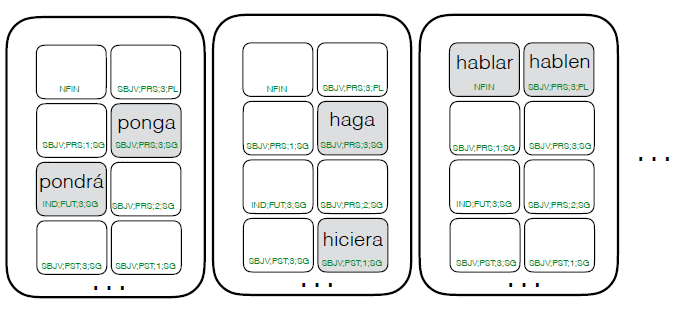
\includegraphics[width=10cm]{figs/PCFP.PNG}
\caption[Paradigm Cell Filling Problem]{Illustration of the Paradigm Cell Filling Problem \citep{silfverberg_encoder-decoder_2018} with Spanish verb paradigms.}
\label{fig:PCFP}
\end{center}
\end{figure}


Other work with supervised learning has attempted to induce inflectional paradigms from text. Paradigms have to be completed by finding overlapping patterns from several incomplete paradigms that are found in text. One method abstracts the longest common subsequence of characters in inflected forms of the same lexeme and then clusters words with same or similar patterns  \citep{ahlberg_semi-supervised_2014,ahlberg_paradigm_2015}. This is illustrated in Figure \ref{fig:LCS}. Exceptions or irregularities in the paradigms can be accounted for by collapsing the similar patterns. The experiment has been quite successful for a few Indo-European languages (German, Spanish, Catalan, French, Galician, Italian, Portuguese, Russian), as well as Maltese and Finnish. Paradigm completion work includes
\citet{malouf_generating_2016}, who trained recurrent neural networks and applied them successfully to Irish, Maltese, and Khaling, among other languages.
\citet{silfverberg_encoder-decoder_2018} also trained neural networks for the task.  \citet{kann-etal-2017-neural} differed from other approaches in that they encoded multiple inflected forms of a lemma to provide complementary information for the generation of unknown forms of the same lemma.
Finally, \citet{cotterell-etal-2017-neural} introduced neural graphical models which completed paradigms based on principal parts.

The unsupervised version of the paradigm completion task \citep{jin2020unsupervised} has been the subject of a recent shared task \citep{kann2020sigmorphon}, with the conclusion that it is extremely challenging for current state-of-the-art systems. 

\begin{figure}[tb]
\begin{center}
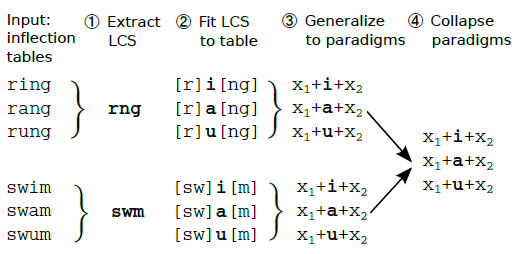
\includegraphics[width=10cm]{figs/Ahlberg2015-LCS.PNG}
\caption[Ahlberg et al. (2015)]{Ahlberg et al. (2015): Inducing paradigms. The longest common subsequences (LCS) \textit{rng} or \textit{swm} are extracted (step 1) and represented as \textit{x\textsubscript{1}} and \textit{x\textsubscript{2}} which replace the LCS (step 2). Words with the same inflectional patterns will be identical (step 3) and can be generalized into paradigms (step 4). The remaining characters \textit{i}, \textit{a}, \textit{u} are assumed to be inflectional affixes.}
\label{fig:LCS}
\end{center}
\end{figure}


Most recent work in the area of paradigm induction has been concerned with generation (as opposed to analysis) of inflected words and has focused on morphological inflection or reinflection. Approaches include \citet{durrett-denero-2013-supervised,nicolai-etal-2015-inflection,faruqui-etal-2016-morphological,kann-schutze-2016-single,aharoni-goldberg-2017-morphological}. Partially building on these, other research has developed machine learning models which are more suitable for low-resource languages and perform well with limited data \citep{kann-etal-2017-one,sharma-etal-2018-iit,makarov-clematide-2018-imitation,wu-cotterell-2019-exact,kann2020learning,wu2020applying}. These are relevant approaches and models for this dissertation, since it aims to aid the documentation and description of low-resource languages. 
%Accordingly, we use the systems by \citet{wu-cotterell-2019-exact} and \citet{wu2020applying} in our experiments.

With formal notation, we can describe the most important generation tasks from the computational morphology literature. 

Formally, paradigm of a lemma~$\ell$ can be denoted as:
\begin{equation}
    \pi(\ell) = \left\langle f(\ell, \vec{t}_\gamma)\right\rangle_{\gamma \in \Gamma(\ell)}
\end{equation}

\noindent where $f : \Sigma^* \times \mathcal{T} \to \Sigma^*$ defines a mapping from a tuple consisting of the lemma and a vector $\vec{t}_\gamma \in \mathcal{T}$ of morphological features to the corresponding inflected form. $\Sigma$ is an alphabet of discrete symbols, i.e., the characters used in the natural language. $\Gamma(\ell)$ is the set of slots in lemma $\ell$'s paradigm. 
We will abbreviate $f(\ell, \vec{t}_\gamma)$ as $f_{\gamma}(\ell)$ for simplicity.


\paragraph{Morphological inflection.}
The task of morphological inflection consists of generating unknown inflected forms, given a lemma 
$\ell$ and a feature vector $\vec{t}_\gamma$. Thus, it corresponds to learning the mapping $f : \Sigma^* \times \mathcal{T} \to \Sigma^*$. Training data consists of lemmas and paradigms.


\paragraph{Morphological reinflection. }
Morphological \textit{re}inflection is a generalized version of the previous task. Here, instead of having a lemma as input, systems are given some \textit{inflected form}  
$f(\ell, \vec{t}_{\gamma_1})$ -- optionally together with $\vec{t}_{\gamma_1}$ -- and a target feature vector $\vec{t}_{\gamma_2}$. The goal is then to produce the inflected form $f(\ell, \vec{t}_{\gamma_2})$. This task is conducted in Chapters \ref{chap:IGT2P} and \ref{chap:POS}.


\paragraph{Paradigm completion. }
The task of paradigm completion consists of, given a \textit{partial} paradigm $\pi_P(\ell) = \left\langle f(\ell, \vec{t}_\gamma)\right\rangle_{\gamma \in \Gamma_P(\ell)}$ of a lemma $\ell$, generating all inflected forms for all slots $\gamma \in \Gamma(\ell) - \Gamma_P(\ell)$.
Training data for this task consists of entire paradigms.

\paragraph{Unsupervised morphological paradigm completion. } For the \textit{unsupervised} version of the paradigm completion task, systems are given a corpus $\mathcal{D}=w_1,\dots,w_{|\mathcal{D}|}$ with a vocabulary $V$ of word types $\{w_i\}$ and a lexicon $\mathcal{L} = \{\ell_j\}$ with $|\mathcal{L}|$~lemmas belonging to the same part of speech. However, no explicit paradigms are observed during training.
The task of unsupervised morphological paradigm completion then consists of
generating the paradigms~$\{\pi(\ell)\}_{\ell\in\mathcal{L}}$ of all lemmas $\ell \in \mathcal{L}$.




\section{POS Tagging and Computational Morphology}
\label{sec:POSlitreview}

Parts of speech (POS), also known as word classes or lexical categories, communicate information about a word, its morphological structure and inflectional paradigm, and its potential grammatical role in a clause. POS tagging is a well-studied problem in NLP. Work on POS tagging has led to the development of several related resources in NLP and linguistics including numerous methods for automatic tagging (e.g. \citet{kupiec_robust_1992,toutanova_bayesian_2008}) as well as tag sets. The most popular tag set for English was developed by the Penn Treebank Project \citep{penn_mitchell_1993}. A universal POS tag set was proposed by \citet{petrov_universal_2012} and has been widely adopted. It closely follows traditional linguistic conventions for common lexical categories as can be seen by comparing to the Leipzig Glossing Rules \citep{leipzig_2008} which also has recommended tags for less common categories.

%\paragraph{Morpheme Segmentation and Glossing.}
%Many NLP models have been applied to automated segmentation and glossing of low-resource languages, but they often tackle just one of the two tasks. Automatic morpheme segmentation was introduced by \citet{harris_phoneme_1970} and much early segmentation research implemented unsupervised learning \citep{goldsmith_unsupervised_2001,creutz_unsupervised_2002,poon_unsupervised_2009}. Supervised models depend on annotated data that is provided by linguists. Published linguistic descriptive data is used usually after some preprocessing. 
%\citet{moeller_automatic_2018} trained a joint segmentation and glossing system on Lezgi using field data.
Work in computational morphology for low-resource languages generally makes the assumption that other interlinear information is available. POS tags are an example of information frequently assumed to be available. For example, 
%\citet{mcmillan-major_automating_2020} trained a conditional random field (CRF) model to produce a gloss line for several high-resource languages and three low-resource languages. The low-resource language data came from interlinearized data that was polished for publication. 
\citet{mcmillan-major_automating_2020} and other experiments such as \citet{samardzic_automatic_2015} assumed information from lines of interlinearized texts such as translation and POS tags. This assumption is also visible in work on morphological inflection paradigm learning or reinflection, such as in the universal presence of POS tags in work developed as part of the SIGMORPHON Shared Tasks. 
